\chapter{Initial Evaluation}\label{C:init_eval}

\section{Initial Experimental Setup at Project Start}
Given that the express purpose of the project is the development of a new version of instrumentation, the first step is an examination of the prior system. This is to identify how it falls short and to determine the areas that the project will focus on.

The experimental method concerns depositing a liquid droplet upon a heated substrate. The data of note is the temperature evolution of the substrate directly under the drop, as well as image data capturing the point of impact and how the droplet changes over the course of the evaporation.

\vspace*{-16pt}
\begin{figure}[h]
    \begin{center}
        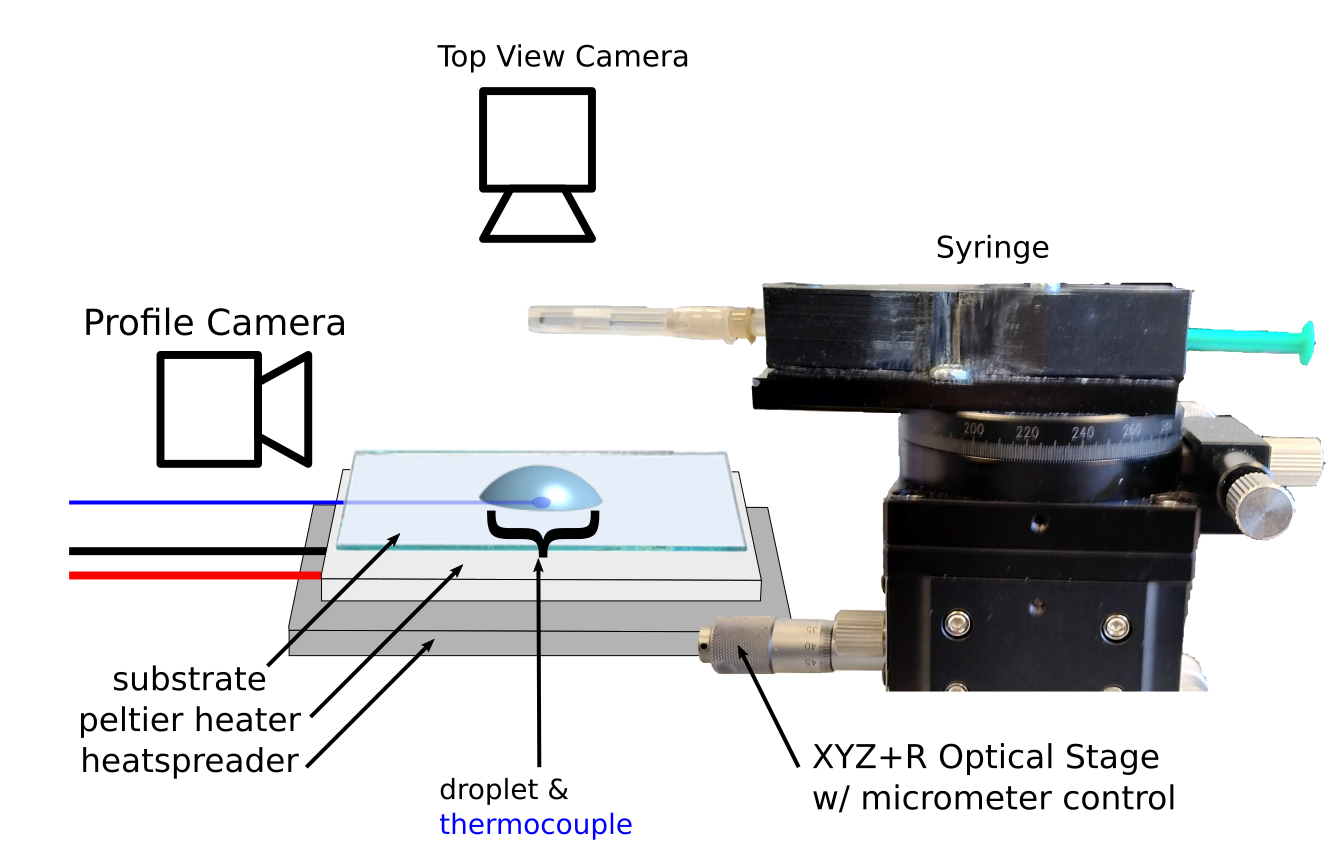
\includegraphics[width=.6\textwidth]{img/init_syr.png}
        \caption{Initial Experimental Setup}
        \label{fig:prior_exp}
    \end{center}
\end{figure}
\vspace*{-16pt}

The prior system uses an optical breadboard and micrometer adjustable stages as mounting platforms and positional control.
A central stage holds the substrate stack, consisting of an aluminium heat-spreader, Peltier heater, and metallic substrate (copper, stainless steel, etc) with an internally mounted thermocouple.
To capture the image data, a pair of manual focus cameras are positioned/suspended in profile and top-down view and are controlled via a USB connection. The thermocouple is sampled with LabVIEW via a USB DaQ.
Dispensing the droplet itself is done by hand using a syringe mounted to another optical stage [\ref{fig:prior_exp}] with XYZ+R controls. It is rotated above the substrate and pressed to dispense a drop.

This would be perfectly fine, however, the results this manual process yields had a level of inconsistency. Thus motivating the design of a new system to control for the experiments variation.

\section{Repeatability and Reliability}
To identify more precisely the drawbacks in the performance of the prior setup and inform the requirements of the project, previously collected data was first analysed.

The data was taken from a series of five droplet runs, and was analysed to quantify the repeatability and reliability of the system and to compare the effect of the drop morphology and position with the resulting temperature evolution.

\begin{figure}[h]
    \centering
    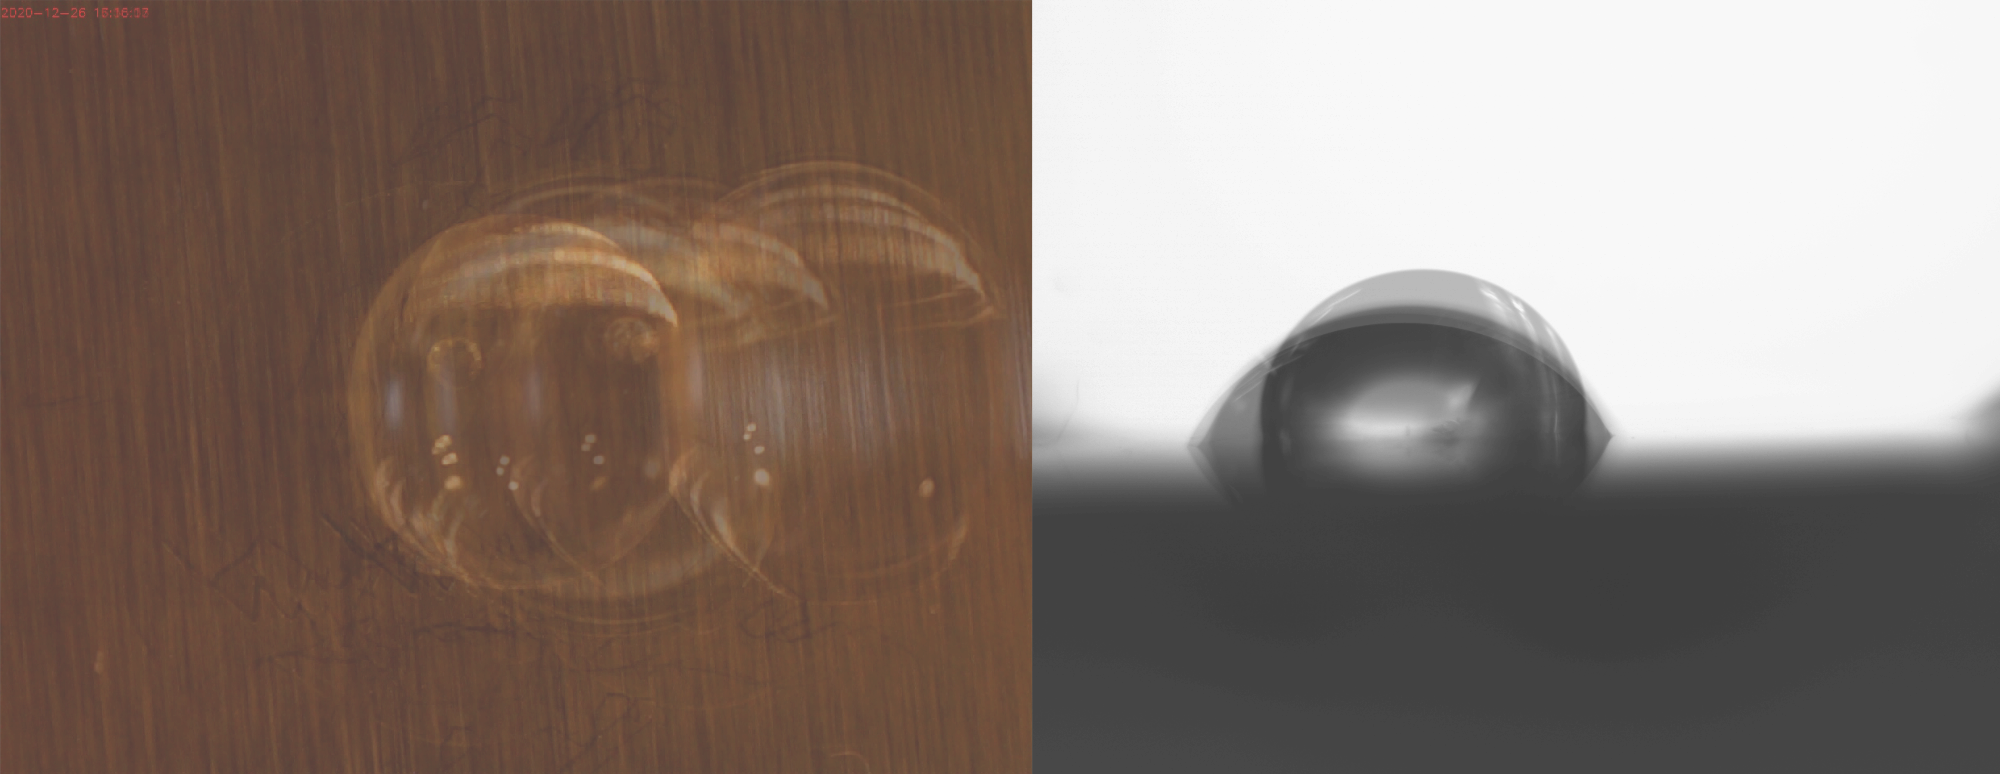
\includegraphics[width=.4\textwidth]{img/droplets_2018.png}
    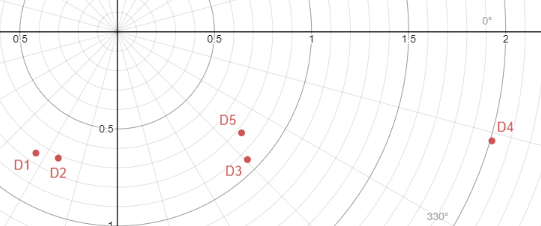
\includegraphics[width=.4\textwidth]{img/drop_pos_2018.png}
    \caption{Droplet positional and shape variation; Left: Camera overlay, Right: Quantified Offsets [mm $\angle$ degrees]}
    \label{fig:init_pos}
\end{figure}

The first analysis is the image data. The substrate itself has a mark to represent the position of the thermocouple, this is used as the main reference to quantify the droplet position. Reference images set calibration at 120.14 pixels/mm and 109.2 pixels/mm for the top down and profile cameras respectively, and was used to measure the droplet centre offset and angle (from the reference point) as well as the height, width and contact angles of the droplet on the substrate.

As seen above, the quite substantial positional variation between the runs. Ranging [0.71:2.01]mm offset and [-16:-123]$^\circ$ angle.


\begin{equation}
    \frac{1}{6}\pi h(3a^2 + h^2)
    : a \equiv \mathrm{half \; width}, \; h \equiv \mathrm{height}
    \label{equ:vol}
\end{equation}
From the data extracted from the profile camera (height, width, contact angle) the volume of the droplets could be estimated. The method chosen was of the represent the droplet as a spherical cap and use the above equation \ref{equ:vol}to compute it.

\begin{figure}[h]
    \centering
    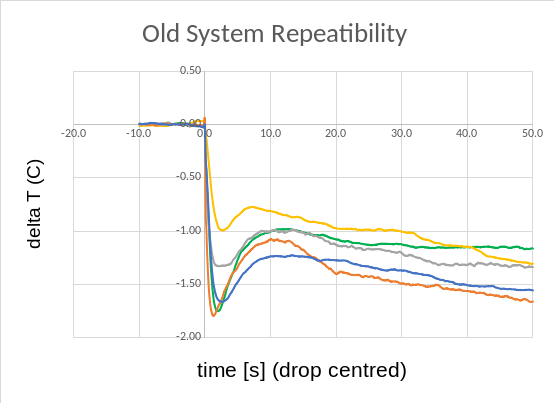
\includegraphics[width=.4\textwidth]{img/drop_temps_2018.png}
    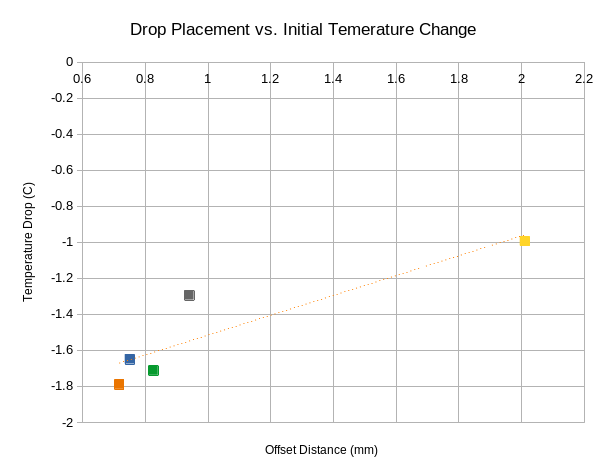
\includegraphics[width=.4\textwidth]{img/2018_pos_temp_trend.png}
    \caption{Left: Initial Systems temperature data showing large relative variation, Right: Drop offset magnitude (mm) against resulting measured temperature drop}
\end{figure}

By taking a series of consecutively collected temperature data using the initial system the observed variation can be quantified. As a pre-processing step a 1sec rolling average is applied to the collected vectors. They are then time aligned to zero at the point of droplet contact, indicated by a sudden temperature drop. This data is then transformed into a temperature delta relative to the temperature just before contact. 

Observed is $0.112^\circ C$ variance between the initial temperature drops between all runs and all runs are observed to evolve at differing rates, rebounding to drifting temperatures etc. This is the main justifying factor in perusing an improved instrumentation system.   

\newpage
\section{Summary}

\begin{table}[h]
    \centering
    \begin{tabular}{|l|l|l|l|}
        \hline
        \textit{\textbf{Droplet}}                          & \textit{Offset(mm)} & \textit{Volume(uL)} & \textit{delta T (c)}\\ \hline
        \cellcolor[HTML]{9698ED}1                          & 0.7506              & 16.55               &  -1.649861        \\ \hline
        \cellcolor[HTML]{E9AD3F}2                          & 0.7164              & 17.91               &  -1.790142        \\ \hline
        \cellcolor[HTML]{C0C0C0}3                          & 0.9402              & 17.89               &  -1.294989        \\ \hline
        \cellcolor[HTML]{FFFC9E}4                          & 2.0104              & 17.57               &  -0.994441        \\ \hline
        \cellcolor[HTML]{79CD5D}5                          & 0.8258              & 16.21               &  -1.712207        \\ \hline
        \cellcolor[HTML]{FFFFFF}\textbf{\textit{Variance}} & \textit{0.2964}     & \textit{0.6288}     &  \textit{0.1121527 }       \\ \hline
    \end{tabular}
\end{table}

To summarise the results of this initial evaluation, a variance of the droplets morphology and resulting temperature measurement are taken and used as a guide for the projects specification and comparative evaluation.    

To fully guide and justify the direction this project will take in attempting to improve this experiment it will consider and address a list of possible affecters on the experiment results.

\begin{table}[h]
    \centering
    \begin{tabular}{|l|l|l|}
        \hline
        \textbf{Effector} & \textbf{Likelihood} & \textbf{Effect Strength} \\ \hline
        Position          & HIGH                & HIGH                     \\ \hline
        Volume            & MODERATE            & HIGH                     \\ \hline
        Contact angle*    & MODERATE            & MODERATE                     \\ \hline
        Humidity          & LOW                 & HIGH                     \\ \hline
        Temperature       & LOW                 & HIGH                     \\ \hline
        Pressure          & MODERATE            & MODERATE                 \\ \hline
    \end{tabular}
\end{table}
\textit{\small{*Contact angle is more a function of the surface cleaning of the substrate, and is only representative of the surface area of contact with the substrate}} \\

Droplet position is a result of the method of dispensing and as seen in figure 3.3 correlates to variation in the observed temperature data collected via the substrates embedded thermocouple. Due to the manual method of dispensing, this variation is very likely to occur and is essentially uncontrolled in the initial experiment other than a reference point as a target. 
The volume and Contact angle of the droplet is more a result of procedural inconsistencies. The volume being a factor of the syringe and contact angle being very dependant of the surface finish/quality/cleaning of the substrate.

The environmental factors differ from these, as the experiment is carried out in a climate-controlled lab there are very few high-frequency changes but these factors can greatly affect the rate of evaporation of the droplet.

Given the above, this project will focus on the controlling the procedural affecters but will supply a method for collecting data on the environmental affecters for analysis.